\documentclass[journal]{IEEEtran}
\usepackage[a5paper, margin=10mm, onecolumn]{geometry}
\usepackage{lmodern}
\usepackage{amsmath, amssymb}
\usepackage{graphicx}
\usepackage{hyperref}
\usepackage{bm} 

\title{8.2.2}
\author{EE24BTECH11004 - Ankit Jainar}
\date{}

\begin{document}

\bibliographystyle{IEEEtran}
\vspace{3cm}

\maketitle

\bigskip

\textbf{Question:}
Find the area bounded by the curves:
\begin{align}
    (x - 1)^2 + y^2 = 1 \quad \text{and} \quad x^2 + y^2 = 1
\end{align}
\newline

\textbf{Theoretical Solution:}

The curves are two circles:
\begin{itemize}
    \item Circle 1: $(x - 1)^2 + y^2 = 1$, centered at $(1, 0)$ with radius $1$.
    \item Circle 2: $x^2 + y^2 = 1$, centered at $(0, 0)$ with radius $1$.
\end{itemize}

\textbf{Step 1: Finding the Points of Intersection}

The points of intersection occur where the two circles overlap. To find the intersection points, we solve the system of equations:
\begin{align}
    (x - 1)^2 + y^2 &= 1 \quad \text{(eq 1)} \\
    x^2 + y^2 &= 1 \quad \text{(eq 2)}
\end{align}

Expanding and simplifying these equations:
\begin{align}
    \text{From Circle 1:} \quad x^2 - 2x + 1 + y^2 &= 1 \\
    \text{From Circle 2:} \quad x^2 + y^2 &= 1
\end{align}

Subtracting the second equation from the first:
\begin{align}
    (x^2 - 2x + 1 + y^2) - (x^2 + y^2) &= 1 - 1 \\
    -2x + 1 &= 0 \quad \implies \quad x = \frac{1}{2}
\end{align}

Substitute $x = \frac{1}{2}$ into the equation of Circle 2:
\begin{align}
    \left(\frac{1}{2}\right)^2 + y^2 &= 1 \\
    \frac{1}{4} + y^2 &= 1 \\
    y^2 &= \frac{3}{4} \quad \implies \quad y = \pm \frac{\sqrt{3}}{2}
\end{align}

Thus, the points of intersection are:
\begin{align}
    P_1 = \left(\frac{1}{2}, \frac{\sqrt{3}}{2}\right), \quad P_2 = \left(\frac{1}{2}, -\frac{\sqrt{3}}{2}\right)
\end{align}

\textbf{Step 2: Theoretical Area Derivation}

The area between the two circles is symmetric about the $x$-axis. Therefore, we calculate the area of the upper region and multiply it by $2$.

\textbf{Integral Setup:}

The area is given by:
\begin{align}
    A = 2 \int_{x=0.5}^{x=1} \left[ \sqrt{1 - (x - 1)^2} - \sqrt{1 - x^2} \right] dx
\end{align}

Here:
\begin{itemize}
    \item $\sqrt{1 - (x - 1)^2}$ represents the upper semicircle of Circle 1.
    \item $\sqrt{1 - x^2}$ represents the upper semicircle of Circle 2.
\end{itemize}

\textbf{Simplify the Expressions:}

Expanding $1 - (x - 1)^2$:
\begin{align}
    1 - (x - 1)^2 &= 1 - (x^2 - 2x + 1) \\
    &= 2x - x^2
\end{align}

Thus, the integral becomes:
\begin{align}
    A = 2 \int_{x=0.5}^{x=1} \left[ \sqrt{2x - x^2} - \sqrt{1 - x^2} \right] dx
\end{align}

\textbf{Numerical Computation:}

The integral can be solved numerically using software tools or approximations. The exact value of the area can be found using such methods.

\textbf{Matrix Representation:}
The system of equations can be represented in matrix form as:
\begin{align}
    \bm{A} \cdot \bm{x} = \bm{b}
\end{align}
where:
\begin{align}
    \bm{A} &= \begin{bmatrix}
        1 & 0 & -1 \\
        1 & 1 & 0
    \end{bmatrix}, \quad
    \bm{x} = \begin{bmatrix}
        x \\
        y^2 \\
        c
    \end{bmatrix}, \quad
    \bm{b} = \begin{bmatrix}
        1 \\
        1
    \end{bmatrix}
\end{align}

Solve for \(\bm{x}\) using Gaussian elimination or matrix inversion:
\begin{align}
    \bm{x} = \bm{A}^{-1} \cdot \bm{b}
\end{align}

\textbf{Step 2: Area Calculation:}
The area between the two circles is given by:
\begin{align}
    A = 2 \int_{x=0.5}^{x=1} \left[ \sqrt{1 - (x - 1)^2} - \sqrt{1 - x^2} \right] dx
\end{align}

Using matrix-based numerical integration, the integral is discretized as:
\begin{align}
    A \approx 2 \cdot h \cdot \sum_{k=0}^{N-1} \left[ f(x_k) - g(x_k) \right]
\end{align}
where:
\begin{align}
    f(x_k) = \sqrt{1 - (x_k - 1)^2}, \quad g(x_k) = \sqrt{1 - x_k^2}
\end{align}

Here, \(x_k\) are discretized points in the range \([0.5, 1]\), and \(h\) is the step size.

\textbf{Step 3: Numerical Integration:}
By substituting the values of \(x_k\) and performing matrix-based summation, the approximate area is calculated. The integral can also be solved symbolically for exact results.


\begin{figure}[h!]
    \centering
    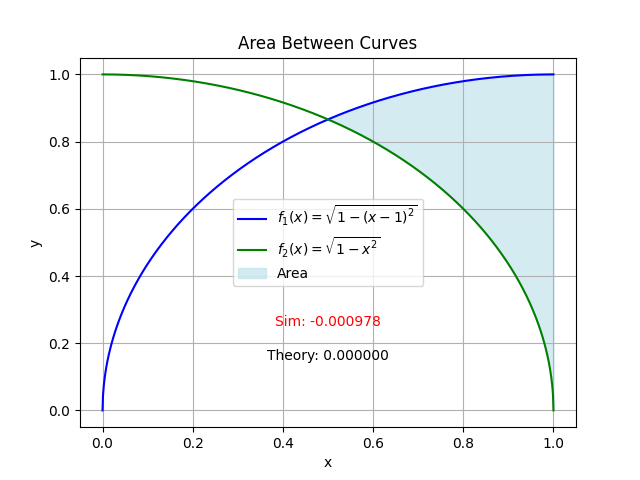
\includegraphics[width=\columnwidth]{figs/fig.png} 
\end{figure}

\end{document}

